\chapter{Linear elasticity and singular problems}
\label{chap-elasticity}

\section{Introduction} 

Let us consider an elastic body $\Omega_0$ that is being deformed under a load
to become $\Omega$.
the deformation $\chi$ of a body in the undeformed state $\Omega_0$ to deformed state $\Omega$. A point in the body has then moved
\begin{align}
u = x - X,
\end{align}
by definition this is \emph{displacement field}. An illustration is shown in Figure \ref{el:def}. 

\begin{figure}[h!]

\begin{center}
  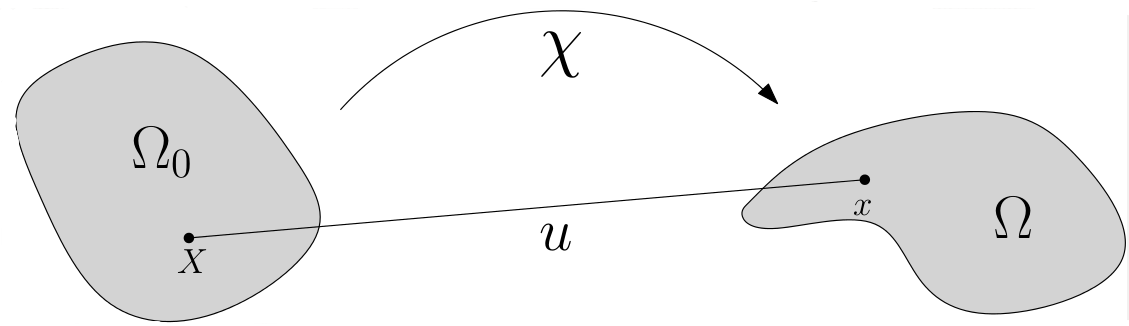
\includegraphics[scale=0.25]{chapters/elasticity/displace.png}
  \end{center}
\caption{Deforming body and displacement vector $u$.}
\label{el:def}
\end{figure}

Here, the domain $\Omega_0 \subset \R^3$. From continuum mechanics, the elastic deformation is modelled by the stress tensor $\sigma$ which is a symmetric $3\times 3$ tensor. 
In equilibrium (i.e. no accelration terms) the Newton's second law states 
the balance of forces as: 
\begin{eqnarray*}  
\operatorname{div} \sigma &=& f, \quad\mbox{in}\ \Omega ,  \\ 
\sigma \cdot n &=& g, \quad\mbox{on}\ \partial \Omega,   
\end{eqnarray*}  
where $f$ and $g$ are body and surface forces,  respectively and $n$ is the outward normal vector.   

For small deformations of an isotropic media, Hooke's law is a good approximation. 
Hooke's law states that 
\[
\sigma = 2 \mu \epsilon(u) + \lambda \operatorname{tr}(\epsilon(u)) \delta.  
\]
Here, $\epsilon(u)$ is the strain tensor or the symmetric gradient: 
\[
\epsilon(u) = \frac{1}{2} (\nabla u + (\nabla u)^T),   
\]
$\mu$ and $\lambda$ are the Lame constants, $\operatorname{tr}$ is the trace operator (the sum of the diagonal matrix
entries), $u$ is the displacement, and  
\[
\delta = \left[ \begin{array}{ccc} 1 & 0 & 0 \\ 0 & 1 & 0 \\ 0 & 0 & 1 \end{array} \right].
\]

From Newton's second law and Hooke's law we arrive directly at the equation of linear elasticity: 
\begin{align}
\label{el:eq}
-2 \mu (\nabla \cdot \epsilon (u)) - \lambda \nabla (\nabla \cdot u) = f.
\end{align}
The equation of linear elasticity \eqref{el:eq} is an elliptic equation, but there are crucial differences between this equation
and a standard elliptic equation like $-\Delta u = f$. These differences often cause
problems in a numerical setting. To explain the numerical issues we will here
focus on the differences between the three operator:
\begin{enumerate}
\item $-\Delta  = \nabla\cdot\nabla  = \operatorname{div}\operatorname{grad} $,
\item $\nabla \cdot \epsilon = \nabla\cdot(\frac{1}{2}(\nabla + (\nabla^T))$,
\item $\nabla \cdot \operatorname{tr} \epsilon = \nabla \nabla \cdot = \operatorname{grad} \operatorname{div}$. 
\end{enumerate}
In particular, the differences between the operators in 1. and 2. is that $\nabla \cdot \epsilon$ has a
larger kernel than $-\Delta$. The kernel consists of rigid motions and this leads to the usage of
of one of Korn's lemmas.
This is the subject of Section \ref{el:korn}. The kernel of the operators  
$\operatorname{grad} \operatorname{div}$ and $\operatorname{div}\operatorname{grad}$
are also different but here in fact the kernel of $\operatorname{grad} \operatorname{div}$ is infinite dimentional
and this has different consequences for the numerical algorithms which not necessarily pick up this kernel at
all. This is discussed in Section \ref{el:lock}.

\section{The operator $\nabla \cdot \epsilon$ and rigid motions}
\label{el:korn}
The challenge with the handling of the $\nabla \cdot \epsilon$ operator is the
handling of the singularity in the case of pure Neumann conditions. Let us therefore
start with the simpler problem of the Poisson problem with Neumann conditions, i.e., 
\begin{eqnarray}
-\Delta u &=& f, \quad \mbox{in}\ \Omega, \\
\frac{\partial u}{\partial n} &=& g, \quad \mbox{on}\ \partial \Omega .
\end{eqnarray}
It is easy to see that this problem is singular: Let $u$ be a solution
of the above equation, then $u+C$ with $C\in\R$ is also a solution because
$-\Delta u = \Delta (u + C) = f$ and
$\frac{\partial u}{\partial n} = \frac{\partial (u+C)}{\partial n} = g$.
Hence, the solution is only determined up to a constant. This means
that  the kernel  is 1-dimentional.

A proper formulation of the above problem can be obtained by using the method
of Lagrange multipliers to fixate the element of the 1-dimentional
kernel. The following weak formulation is well-posed:
Find $u\in H^1$ and $\lambda \in \R$ such that
\begin{eqnarray}
\label{poisson:neu1}
a(u,v) + b(\lambda, v) &=& f(v) \quad \forall v\in H^1 \\
\label{poisson:neu2}
b(u, \gamma) &=& 0, \quad \forall \gamma \in \R.
\end{eqnarray}
Here,
\begin{eqnarray}
\label{poisson:neu3}
a(u,v) &=& (\nabla u, \nabla v), \\
\label{poisson:neu4}
b(\lambda, v) &=& (\lambda, v), \\
\label{poisson:neu5}
f(v) &=& (f,v) + \int_{\partial \Omega} g v ds .
\end{eqnarray}
Hence, the method of Lagrange multipliers turns the original problem
into a saddle problem similar that in Chapter \ref{chap-stokes}. However,
in this case the Brezzi conditions are easily verified. We remark
however that this formulation makes the problem indefinite rather
than positive definite and for this reason alternative techniques
such as pin-pointing is often used instead. We will not avocate this
approach as it often causes numerical problems. Instead, we
include a code example that demonstrate how this problem can
be implemented with the method of Lagrange multipliers in FEniCS.
\begin{python}
from dolfin import *

mesh = UnitSquareMesh(64, 64)

# Build function space with Lagrange multiplier
P1 = FiniteElement("Lagrange", mesh.ufl_cell(), 1)
R = FiniteElement("Real", mesh.ufl_cell(), 0)
W = FunctionSpace(mesh, P1 * R)

# Define variational problem
(u, c) = TrialFunction(W)
(v, d) = TestFunctions(W)
f = Expression("10*exp(-(pow(x[0] - 0.5, 2) + pow(x[1] - 0.5, 2)) / 0.02)", degree=2)
g = Expression("-sin(5*x[0])", degree=2)
a = (inner(grad(u), grad(v)) + c*v + u*d)*dx
L = f*v*dx + g*v*ds

# Compute solution
w = Function(W)
solve(a == L, w)
(u, c) = w.split()

# Plot solution
plot(u, interactive=True)
\end{python}

The kernel of the $\epsilon$ operator is the space of rigid motions, $\operatorname{RM}$. The space consists of translations and rotations. Rigid motions
are on the following form in 2D and 3D:
\begin{eqnarray}
\operatorname{RM}_{2D} &=& \left[\begin{array}{c} a_0 \\ a_1 \end{array}\right] + a_2 \left[\begin{array}{c} -y\\ x\end{array} \right], \\
\operatorname{RM}_{3D} &=& \left[\begin{array}{c} a_0 \\ a_1 \\ a_2 \end{array}\right]
     + \left[\begin{array}{ccc} 0 & a_3 & a_4 \\
                               -a_3 & 0 & a_5\\
                               -a_4 & -a_5 & 0
             \end{array}\right]
 \left[\begin{array}{c}
x\\ y \\ z \end{array} \right].
\end{eqnarray}
Hence, the kernel in 2D is three-dimentional and may be expressed as above in terms of the degrees of freedom $(a_0, a_1, a_2)$ whereas the kernel in 3D is six-dimentional $(a_0, \ldots, a_5)$.

The Korn's lemmas states suitable conditions for solvability. Here, we include two of the three inequalities typically
listed.  
\begin{itemize}
\item The first lemma: For all $u\in H^1 \backslash \operatorname{RM}$ we have that $\|\epsilon(u)\| \ge C \|u\|_1$.
\item The second lemma: For all $u\in H^1_0 $ we have that $\|\epsilon(u)\| \ge C \|u\|_1$. 
\end{itemize}
These lemmas should be compared with the Poincare's lemma and the equivalence of the $|\cdot|_1$ and $\|\cdot\|_1$ norms.
The second lemma states that when we have homogenous Dirichlet conditions we obtain a well-posed problem
in a similar manner as for a standard elliptic problem. This case is often called fully-clamped conditions.
For the Neumann problem, however, coersivity is not obtained unless we remove the complete set of rigid motions
for the function space used for trial and test functions. Removing the rigid motions is most easily done
by using the method of Lagrange multipliers. 

Let us now consider a weak formulation of the linear elasticity problem and describe how to implement
it in FEniCS. For now we consider the case where $\lambda$ and $\mu$ are of comparable magnitude. In
the next section we consider the case where $\lambda \gg \mu$.
The weak formulation of the linear elasticity problem is:
Find $u\in H^1$ and $r \in \operatorname{RM}$ such that
\begin{eqnarray}
\label{el:lm:1}
a(u,v) + b(r, v) &=& f(v), \quad \forall v\in H^1, \\
\label{el:lm:2}
b(s,u) &=& 0, \quad \forall s \in \operatorname{RM}.
\end{eqnarray}
Here,
\begin{eqnarray}
a(u,v) &=& \mu (\epsilon(u), \epsilon(v)) + \lambda (\operatorname{div} u, \operatorname{div} v)  \\
b(r, v) &=& (r, v), \\
f(v) &=& (f,v) + \int_{\partial \Omega} g v ds .
\end{eqnarray}

As we know from Chapter \ref{chap-stokes}, this is a saddle point problem and we need to
comply with the Brezzi conditions. Verifying these conditions are left as Exercise \ref{ex:kornbrezzi}.

\begin{example}
Our brain and spinal cord is floating in a water like fluid called the cerebrospinal fluid.
While the purpose of this fluid is not fully known, it is known that the pressure in
the fluid oscillates with about 5-10 mmHg during a cardic cycle which is approximately one
second, c.f., e.g., ~\cite{eide2016correlation}. The Youngs' modulus has been estimated 16 kPa
and 1 mmHg $\approx$ 133 Pa, c.f., e.g., ~\cite{stoverud2016poro}. To compute the deformation of the brain during a
cardiac cycle we consider solve the linear elasticity problem with Neumann condtions
set as pressure of 1 mm Hg and ... The following code shows the implmentation in FEniCS.
The mesh of the brain was in this case obtained from a T1 magnetic ressonance image
and segmentation was performed by using FreeSurfer. 

\begin{python}
from fenics import *

mesh = Mesh('mesh/res32.xdmf')	# mm

plot(mesh,interactive=True)

# Since the mesh is in mm pressure units in pascal must be scaled by alpha = (1e6)**(-1)
alpha = (1e6)**(-1)

# Mark boundaries
class Neumann_boundary(SubDomain):
	def inside(self, x, on_boundry):
		return on_boundry

mf = FacetFunction("size_t", mesh)
mf.set_all(0)

Neumann_boundary().mark(mf, 1)
ds = ds[mf]

# Continuum mechanics
E = 16*1e3 *alpha
nu = 0.25
mu, lambda_ = Constant(E/(2*(1 + nu))), Constant(E*nu/((1 + nu)*(1 - 2*nu)))
epsilon = lambda u: sym(grad(u))

p_outside = 133 *alpha
n = FacetNormal(mesh)
f = Constant((0, 0, 0))

V = VectorFunctionSpace(mesh, "Lagrange", 1)

# --------------- Handle Neumann-problem --------------- #
R = FunctionSpace(mesh, 'R', 0)        		 # space for one Lagrange multiplier
M = MixedFunctionSpace([R]*6)          		 # space for all multipliers
W = MixedFunctionSpace([V, M])
u, rs = TrialFunctions(W)
v, ss = TestFunctions(W)

# Establish a basis for the nullspace of RM
e0 = Constant((1, 0, 0))				# translations
e1 = Constant((0, 1, 0))
e2 = Constant((0, 0, 1))

e3 = Expression(('-x[1]', 'x[0]', '0')) # rotations
e4 = Expression(('-x[2]', '0', 'x[0]'))
e5 = Expression(('0', '-x[2]', 'x[1]'))
basis_vectors = [e0, e1, e2, e3, e4, e5]

a = 2*mu*inner(epsilon(u),epsilon(v))*dx + lambda_*inner(div(u),div(v))*dx
L = inner(f, v)*dx + p_outside*inner(n,v)*ds(1)

# Lagrange multipliers contrib to a
for i, e in enumerate(basis_vectors):
	r = rs[i]
	s = ss[i]
	a += r*inner(v, e)*dx + s*inner(u, e)*dx

# -------------------------------------------------------- #

# Assemble the system
A = PETScMatrix()
b = PETScVector()
assemble_system(a, L, A_tensor=A, b_tensor=b)

# Solve
uh = Function(W)
solver = PETScLUSolver('mumps') # NOTE: we use direct solver for simplicity
solver.set_operator(A)
solver.solve(uh.vector(), b)

# Split displacement and multipliers. Plot
u, ls = uh.split(deepcopy=True) 
plot(u, mode='displacement', title='Neumann_displacement',interactive=True)

file = File('deformed_brain.pvd')
file << u 

\end{python}
\end{example}

\begin{figure}[h!] 
\begin{center}
  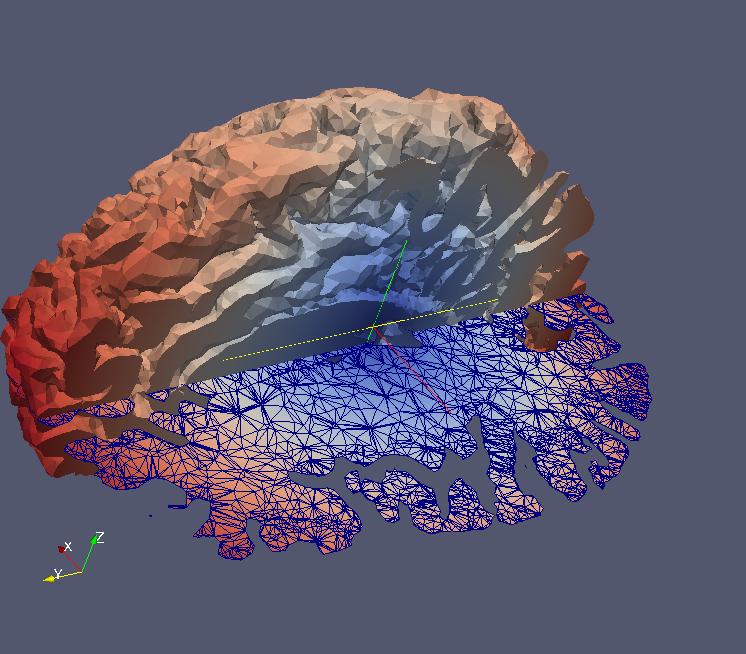
\includegraphics[scale=0.25]{chapters/elasticity/screen_shot.png}
  \end{center}
\caption{Deformation of the human brain during a cardiac cycle.}
\end{figure}


\section{Locking}
\label{el:lock}
The locking phenomena has nothing to do with the problem related to the rigid motions
studied in the previous section. Therefore, we consider locking in the simplest case possible
where we have homogenous Dirichlet conditions. In this case the elasticity equation
can be reduced to
\begin{eqnarray*}
-\mu \Delta u - (\mu + \lambda) \nabla \nabla\cdot u &=& f, \quad \mbox{in} \Omega,\\
                                                   u &=& 0, \quad \mbox{on} \partial \Omega. 
\end{eqnarray*}
The weak formulation of the problem then becomes:
Find $u \in H^1_0$ such that
\[
a(u,v) = f(v), \quad \forall v \in H^1_0, 
\]
where
\begin{eqnarray}
a(u,v) &=& \mu (\nabla u, \nabla v) + (\mu + \lambda) (\nabla \cdot u, \nabla \cdot v),\\
f(v)   &=& (f, v) .
\end{eqnarray}

The phenomen locking is a purely numerical artifact that arise when $\lambda \gg \mu$.
Roughly speaking, approximating $\nabla$ and $\nabla\cdot$ require different methods.
While vertices based approximations work fine for $\nabla$, edge based methods
are more natural for $\nabla\cdot$ since this operator relates directly
to the flux through the element edges.

For smooth functions, it can be verified directly that
\[
\Delta = \nabla\cdot\nabla = \nabla\nabla\cdot + \nabla\times \nabla\times
\]
where $\nabla\times$ is the curl operator.
Hence in $H_0^1$ we have 
\[
(\nabla u,\nabla v) = (\nabla \cdot u,\nabla \cdot v) + (\nabla \times u,\nabla \times v).
\]

Furthermore, it is well known (the Helmholz decomposition theorem) that any field in $L^2$ or $H^1$ can be decomposed
into a the gradient of a scalar potential (irrotational, curl-free vector field)
and the curl of scalar (a solenoidal, divergence-free vector field). That is,
\[
u = \nabla \phi + \nabla \times \psi, 
\]
where $\phi$ and $\psi$ are scalar fields that can be determined. 
Furthermore, 
\begin{eqnarray}
\nabla\cdot\nabla\times u = 0, \\
\nabla\times\nabla\cdot u = 0. 
\end{eqnarray}
This means that
\[
\nabla\nabla\cdot u = \left\{ \begin{array}{cc}
                          \Delta u & \mbox{ if } u \mbox{ is a gradient} \\
                                             0  & \mbox{ if } u \mbox{ is a curl}
                          \end{array} \right. 
\]
As the material becomes incompressible, when $\lambda\rightarrow\infty$ the gradient
part is being locked and $\phi$ tends to zero. However, the curl represented by $\psi$
remains unaffected. Vertex based finite elements such as Lagrange are poor
at distinguising between gradients and curls and tend to lock the complete solution.
Exercise \ref{ex:lock} investigates this phenomena numerically.

To avoid locking it is common to introduce a the quantity solid pressure,
$p = (\mu + \lambda) \nabla \cdot u$. Introducing this as a separate
unknown into the system we obtain the equations:
\begin{eqnarray*}
-\mu \Delta u - \nabla p = f, \\
\nabla\cdot u - \frac{1}{\mu + \lambda} p = 0 . 
\end{eqnarray*}
This system of equations is similar to the Stokes problem.
Hence, we may formulation a weak problems as follows.
Find $u\in H^1_0$ and $p \in L^2$ such that
\begin{eqnarray}
a(u,v) + b(p, v) &=& f(v) \forall v\in H^1 \\
b(u, q) - c(p,q) &=& 0, \forall q \in \R.
\end{eqnarray}
Here,
\begin{eqnarray}
a(u,v) &=& (\nabla u, \nabla v), \\
b(p, v) &=& (\nabla p, v), \\
c(p,q) &=& \frac{1}{\mu + \lambda}(p,q)\\
f(v) &=& (f,v).
\end{eqnarray}

The case when $\lambda\rightarrow\infty$ then represents the Stokes
problem as $\frac{1}{\mu + \lambda}\rightarrow 0$. Hence, for this
problem we know that stable discretizations can be obtained
as long as we have Stokes-stable elements like for instance Taylor--Hood.
We also remark that Stokes-stable elements handle any $\mu, \lambda$
because the $-c(p,q)$ is a negative term that only stabilize.
In fact, this problem is identical to the proposed penalty
method that was discussed for the Stokes problem. 



\begin{exercise}
\label{ex:sym:tensor}
Show that the inner product of a symmetric matrix $A$ and matrix $B$ equals
the inner product of $A$ and the symmetric part of $B$, i.e., that
$A:B$ = $A:B_S$, where $B_S = \frac{1}{2} (B + B^T)$. 
\end{exercise}

\begin{exercise}
Show that the term $\operatorname{div} \epsilon(u)$ in a weak setting may be written as $(\epsilon(u), \epsilon(v))$. Use the result of Exercise \ref{ex:sym:tensor}.   
\end{exercise}

\begin{exercise}
\label{ex:poissonbrezzi}
Show that the Brezzi conditions (\ref{remark1}-\ref{remark4}) for the singular problem of homogenous Neumann conditions for the Poisson problem \eqref{poisson:neu1}--\eqref{poisson:neu5}. Hint: use the following version of Poincare's lemma: 
\[
\|u-\bar{u}\|_0 \le C \|\nabla u \|_0, \quad \forall u \in H^1 .  
\]
Here, $\bar{u}=\frac{1}{|\Omega|}\int_\Omega u dx$. 
As always, the inf-sup condition is challenging, but notice that
\[
sup_{u\in V_h} \frac{b(u,q)}{\|u\|_{V_h}} \ge \frac{b(\bar{u},q)}{\|\bar{u}\|_{V_h}} .  
\]
\end{exercise}



\begin{exercise}
\label{ex:kornbrezzi}
Show that three of Brezzi conditions (\ref{remark1}-\ref{remark3}) for problem linear elasticity problem with pure Neumann conditions \eqref{el:lm:1}-\eqref{el:lm:2} are valid. Hint: use Korn's lemma for the coersivity.
As always, the inf-sup condition is challenging and we refer to \cite{kuchta2016singular}.
\end{exercise}

\begin{exercise}
\label{ex:lock}
We will consider the topic 'locking'. 
Consider the following equation on the domain $\Omega=(0,1)^2$: 
\begin{eqnarray}
-\mu \Delta u - \lambda \nabla \nabla \cdot u   &=& f \mbox{ in } \Omega, \\ 
        u &=& u_{analytical} \mbox{ on } \partial \Omega
\end{eqnarray}
where $u_{analytical}= (\frac{\partial \phi}{\partial y}, -\frac{\partial \phi}{\partial x})$ 
and $\phi= sin(\pi x y)$. Here, by construction, 
$\nabla \cdot u_{analytical} = 0$.  

\noindent
\textbf{a)} 
Derive an expression for $f$. Check that the expression is independent of $\lambda$. 

\noindent
\textbf{b)} 
Compute the numerical error for $\lambda=1, 100, 10000$
at $h=8, 16, 32, 64$ for polynomial order both 1 and 2.  

\noindent
\textbf{c)} 
Compute the order of convergence for different $\lambda$. 
Is locking occuring?

\end{exercise}
